\documentclass[conference,a4paper]{IEEEtran}
\IEEEoverridecommandlockouts
\usepackage[utf8]{inputenc}
\usepackage[T1]{fontenc}
\usepackage{graphicx}
\usepackage{amsmath,amssymb}
\usepackage{booktabs}
\usepackage{multirow}
\usepackage{array}
\usepackage{url}
\usepackage{cite}
\usepackage{balance}
\usepackage{stfloats}
\usepackage[font=footnotesize]{caption}
\usepackage{subcaption}

\newcommand{\RGB}{I_{\mathrm{RGB}}}
\newcommand{\IR}{I_{\mathrm{IR}}}
\newcommand{\Iavg}{I_{\mathrm{avg}}}
\newcommand{\Ia}{I_{\mathrm{A7}}}
\newcommand{\G}{G_{\uparrow}}

\title{Cross-Modal JEPA Gate-Blend Fusion for Lightweight RGB/Infrared Detection and Semantic Segmentation}

\author{\IEEEauthorblockN{Erol Külüşlü}
\IEEEauthorblockA{Department of Electrical-Electronics and Computer Engineering\\
Abdullah Gül University, Kayseri, Turkey\\
Email: akuluslu54@gmail.com}}

\begin{document}
\maketitle

\begin{abstract}
Visible-spectrum perception degrades under night, fog, rain, smoke, and illumination shift, while thermal infrared sensors preserve complementary target information but lack color and fine texture. This work studies whether a lightweight cross-modal fusion module can improve downstream object detection and semantic segmentation when the downstream models are kept small and unmodified. A dual-branch RGB/IR fusion architecture with channel attention, spatial gating, and a cross-modal joint-embedding predictive architecture (CM-JEPA) objective is evaluated on a real RGB/IR manifest containing 6025 aligned pairs from M3FD, MSRS, and RoadScene. Detection is evaluated with YOLO11n on M3FD, segmentation with U-Net/MobileNetV2 on MSRS, and fusion quality with entropy, spatial frequency, average gradient, and normalized mutual information. The final implementation uses a gate-guided representation, \(\Ia=\G \odot \RGB + (1-\G)\odot \mathrm{rep}(\IR)\), because direct use of the raw decoder output caused visual collapse. Results show that fusion is beneficial but that the simplest average fusion is the most stable overall method. Average fusion achieved the best detection mAP@0.5 (0.7718), best mAP@0.5:0.95 (0.5115), and best segmentation mIoU (0.5551). The proposed CM-JEPA gate-blend model was competitive for detection (mAP@0.5:0.95 = 0.5080), but underperformed in segmentation (mIoU = 0.4774). The study therefore supports RGB/IR fusion for lightweight perception, but also shows that classical fusion metrics and learned fusion complexity do not automatically translate into stronger downstream performance.
\end{abstract}

\begin{IEEEkeywords}
RGB-infrared fusion, joint-embedding predictive architecture, attention, YOLO11, U-Net, semantic segmentation, object detection, lightweight perception.
\end{IEEEkeywords}

\section{Introduction}
Robust visual perception is a central requirement for intelligent transportation, surveillance, autonomous mobile robots, and campus-scale monitoring systems. A visible RGB camera captures rich texture, color, and edge information, but it is highly dependent on illumination and is vulnerable to low light, rain, fog, smoke, glare, and other adverse conditions. Infrared (IR) sensing, in contrast, detects thermal radiation and can reveal pedestrians, vehicles, and other heat-related targets when visible imagery becomes unreliable. However, IR imagery usually has lower texture richness, limited semantic color cues, and sometimes weaker object boundaries. These complementary strengths motivate infrared-visible image fusion (IVIF), where RGB and IR streams are combined into a representation that is intended to improve human interpretability and downstream computer vision.

Most IVIF research has focused on image-level quality or on relatively heavy architectures. DenseFuse introduced a deep autoencoder paradigm for IVIF \cite{li2019densefuse}. Task-aware methods such as SeAFusion and TarDAL explicitly connected fusion to high-level vision tasks including segmentation and object detection \cite{tang2022seafusion,liu2022tardal}. More recent approaches such as CDDFuse and MRFS introduced decomposition, correlation, and mutually reinforcing task constraints \cite{zhao2023cddfuse,zhang2024mrfs}. Parallel work in RGB-X perception, such as CMX, demonstrated the value of cross-modal interaction for semantic segmentation \cite{zhang2023cmx}. Despite this progress, an important practical question remains: do learned RGB/IR fusion mechanisms help when the downstream models are lightweight, the evaluation is task-driven, and the same fused image must serve both object detection and semantic segmentation?

This work addresses that question through a controlled comparison study. A cross-modal attention-based fusion model is implemented with dual encoders, SE-style channel attention \cite{hu2018senet}, spatial gating inspired by attention modules such as CBAM \cite{woo2018cbam}, and a JEPA-style representation prediction objective \cite{assran2023ijepa}. The model is compared with RGB-only, IR-only, and average fusion baselines. Instead of evaluating only classical fusion metrics, the fused representations are used as inputs to two lightweight downstream models: YOLO11n for detection \cite{ultralytics2024yolo11} and U-Net with a MobileNetV2 encoder for segmentation \cite{ronneberger2015unet,sandler2018mobilenetv2}. The final report revises the original proposal by incorporating real experimental outcomes from the final Colab implementation.

The contributions are as follows:
\begin{itemize}
    \item A complete real-data RGB/IR fusion pipeline was built and evaluated over 6025 aligned pairs from M3FD, MSRS, and RoadScene.
    \item The study compares RGB-only, IR-only, average fusion, learned attention fusion variants, and the final CM-JEPA gate-blend representation under the same evaluation framework.
    \item Detection and segmentation are evaluated with lightweight downstream models, making the results relevant to edge-oriented perception rather than only image-fusion benchmarking.
    \item The analysis shows that average fusion is the strongest overall baseline, while CM-JEPA gate-blend is detection-competitive but segmentation-weak.
    \item A corrected A7 evaluation protocol is introduced: the CM-JEPA representation is measured using the same gate-blend image used by downstream tasks, not the collapsed raw decoder output.
\end{itemize}

\begin{figure*}[t]
    \centering
    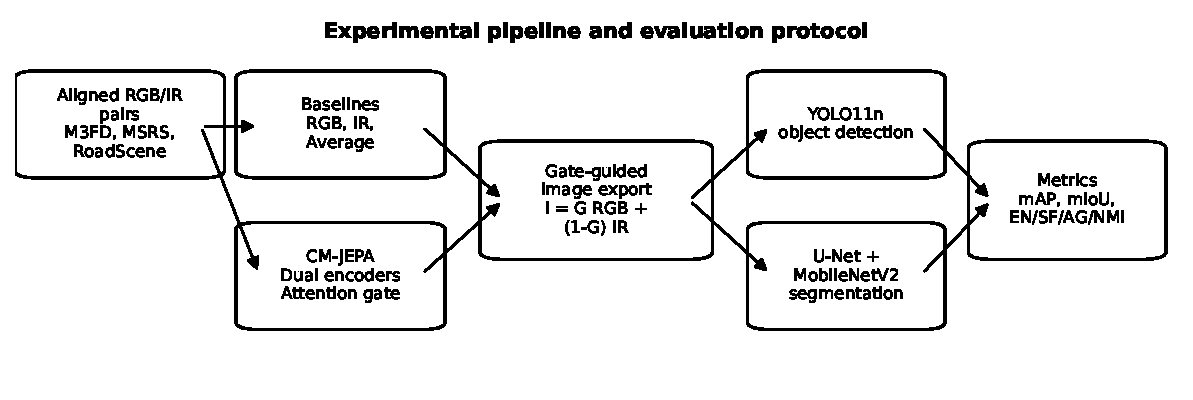
\includegraphics[width=0.96\textwidth]{figures/figure_pipeline.pdf}
    \caption{End-to-end experimental pipeline. RGB/IR data are standardized into paired manifests, evaluated through classical baselines and the proposed CM-JEPA gate-blend representation, and then tested with both image-level fusion metrics and downstream lightweight perception tasks.}
    \label{fig:pipeline}
\end{figure*}

\section{Related Work}
\subsection{Classical and Deep Infrared-Visible Fusion}
Classical fusion methods such as Laplacian pyramid fusion decompose images into multi-scale representations and combine coefficients with deterministic rules \cite{burt1983laplacian}. These methods are simple, transparent, and parameter-free, but they cannot adapt to task-specific semantics. Deep learning methods shifted IVIF toward data-driven feature extraction. DenseFuse used an autoencoder with dense connections to reconstruct fused images from visible and infrared features \cite{li2019densefuse}. Later, CDDFuse decomposed features into modality-shared and modality-specific components and used correlation-driven constraints to improve decomposition quality \cite{zhao2023cddfuse}. These works improved visual fusion quality, but their metrics do not always guarantee improved detection or segmentation.

\subsection{Task-Aware Fusion}
Task-aware fusion explicitly optimizes for high-level perception. SeAFusion connected image fusion with semantic segmentation so that semantic supervision could guide the fusion network \cite{tang2022seafusion}. TarDAL introduced target-aware dual adversarial learning and the M3FD benchmark for detection-oriented fusion \cite{liu2022tardal}. MRFS further coupled fusion and segmentation with mutual reinforcement \cite{zhang2024mrfs}. These works motivate the central design choice of this project: a fusion method should not be judged only by entropy or contrast, but by whether it improves downstream perception.

\subsection{Cross-Modal Attention and Lightweight Perception}
Attention mechanisms are natural tools for RGB/IR fusion because the reliability of each modality varies spatially and semantically. SE-Net recalibrates channels according to global statistics \cite{hu2018senet}, while CBAM sequentially applies channel and spatial attention \cite{woo2018cbam}. CMX generalizes cross-modal transformer fusion to RGB-X segmentation \cite{zhang2023cmx}. In this project, the attention block is kept deliberately lightweight so that the downstream models can remain small. YOLO11n is used as the detection model, and U-Net/MobileNetV2 is used as the segmentation model. This emphasizes whether fusion helps practical lightweight perception, not whether a large downstream architecture can hide weaknesses in the fusion representation.

\subsection{JEPA-Style Self-Supervision}
Joint-embedding predictive architectures learn representations by predicting latent target representations from context representations rather than reconstructing pixels directly \cite{assran2023ijepa}. This idea is attractive for RGB/IR fusion because it can encourage semantic consistency across modalities. However, this project found an important implementation caveat: the raw decoder image of a CM-JEPA fusion module can visually collapse. Therefore, the final representation uses the learned gate for RGB/IR blending rather than the raw decoder output. This is not merely a cosmetic choice; it is essential for valid downstream evaluation.

\section{Materials and Methods}
\subsection{Datasets and Standardized Manifest}
The final real-data manifest contains 6025 aligned RGB/IR pairs. The dataset composition is shown in Fig.~\ref{fig:data}. M3FD contributes 4280 pairs and is used for object detection with six YOLO classes: people, car, bus, motorcycle, truck, and lamp. MSRS contributes 1524 standardized pairs, among which 1444 valid mask-bearing samples are used for segmentation. RoadScene contributes 221 paired samples for fusion-quality and general fusion analysis. The overall manifest split contains 4215 training, 902 validation, and 908 test pairs. For the M3FD detection subset, the saved YOLO split contains 2994 training, 641 validation, and 645 test images for each RGB, IR, average, and proposed representation.

\begin{figure}[t]
    \centering
    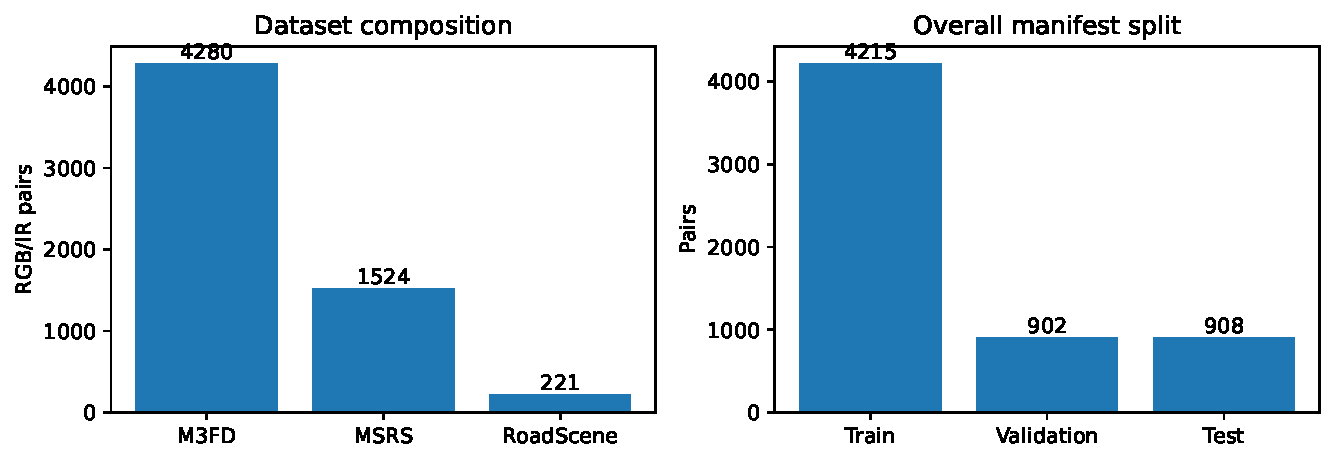
\includegraphics[width=\columnwidth]{figures/figure_dataset_counts.pdf}
    \caption{Dataset and split statistics after standardization. The real-data manifest contains 6025 RGB/IR pairs across M3FD, MSRS, and RoadScene.}
    \label{fig:data}
\end{figure}

\subsection{Baselines}
Four downstream inputs are compared. RGB-only uses the visible image directly:
\begin{equation}
I_{A0}=\RGB .
\end{equation}
IR-only replicates the infrared image into three channels:
\begin{equation}
I_{A1}=\mathrm{rep}(\IR).
\end{equation}
Average fusion computes a simple pixel-level combination:
\begin{equation}
I_{A2}=\frac{1}{2}\RGB + \frac{1}{2}\mathrm{rep}(\IR).
\label{eq:avg}
\end{equation}
This average baseline is intentionally simple. If a learned fusion method cannot outperform it, its complexity must be justified through other advantages such as robustness or task specificity.

\subsection{Proposed CM-JEPA Gate-Blend Fusion}
The proposed model uses two modality-specific encoders, channel attention, and a spatial gate. Let \(F_R\) and \(F_I\) be RGB and IR feature tensors. Channel attention produces recalibrated features \(F'_R\) and \(F'_I\). A spatial gate is then estimated as
\begin{equation}
G = \sigma\left(\phi([F'_R,F'_I])\right),
\end{equation}
where \([\cdot,\cdot]\) denotes concatenation, \(\phi\) is a lightweight convolutional gate predictor, and \(\sigma\) is the sigmoid function. The latent fusion is
\begin{equation}
F_{ctx}=G\odot F'_R+(1-G)\odot F'_I.
\label{eq:latentfusion}
\end{equation}
The initial implementation decoded \(F_{ctx}\) into a 3-channel image through a feature adapter. During evaluation, however, the raw decoder image could collapse into a low-variance gray output. The final code therefore uses the gate consistently at image level:
\begin{equation}
\Ia=\G\odot\RGB+(1-\G)\odot\mathrm{rep}(\IR),
\label{eq:gateblend}
\end{equation}
where \(\G\) is the upsampled spatial gate. This representation is used for YOLO, U-Net, and the repaired A7 fusion-quality metrics.

\begin{figure}[t]
    \centering
    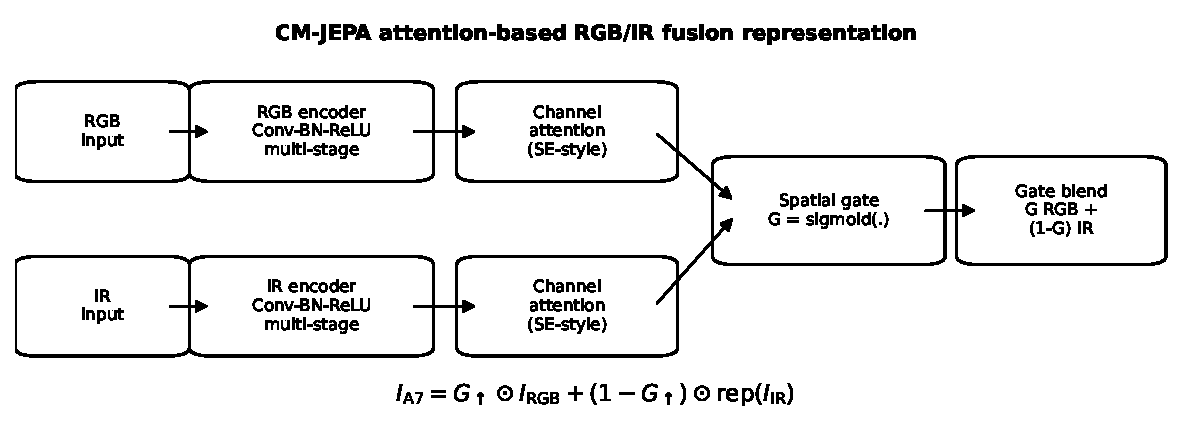
\includegraphics[width=\columnwidth]{figures/figure_architecture.pdf}
    \caption{Simplified architecture of the final proposed representation. The final downstream input is a gate-guided RGB/IR blend rather than the raw decoder output.}
    \label{fig:arch}
\end{figure}

\subsection{Losses and Training Objectives}
The fusion module is trained with a fusion loss and a JEPA-style representation loss. The fusion loss contains intensity and gradient terms:
\begin{equation}
\mathcal{L}_{fus}=\|I_f-I_{ref}\|_1+\lambda_g\|\nabla I_f-\nabla I_{ref}\|_1,
\end{equation}
where \(I_{ref}\) is a modality-derived reference target and \(\lambda_g=5.0\) in the final configuration. The JEPA component predicts target latent tokens from context tokens:
\begin{equation}
\mathcal{L}_{jepa}=\|p(z_c)-\mathrm{sg}(z_t)\|_2^2,
\end{equation}
where \(p(\cdot)\) is a predictor and \(\mathrm{sg}\) denotes stop-gradient. Variance and covariance regularizers are included with weights \(0.05\) and \(0.005\), respectively, to reduce representation collapse. The final notebook uses AdamW with learning rate \(2\times 10^{-4}\), weight decay \(10^{-4}\), EMA momentum 0.996, mask ratio 0.35, base channels 32, latent channels 512, attention reduction 16, and token dimension 256.

\subsection{Downstream Evaluation}
Detection uses YOLO11n with image size 640, batch size 8, and 40 epochs. RGB, IR, and average YOLO checkpoints were loaded from prior successful Drive results rather than retrained. The proposed gate-blend YOLO model was trained on the corrected fused export. Segmentation uses U-Net with a MobileNetV2 encoder, ImageNet initialization, 9 classes, 480\(\times\)640 input, AdamW at \(10^{-4}\), batch size capped at 4, and 40 epochs. Proposed segmentation images are cached once and reused across epochs. The final code cell referenced in this submission is the Colab notebook \cite{kulusslu2026notebook}; the crucial correction is that A7 fusion metrics and downstream inputs are computed from Eq.~\eqref{eq:gateblend}, not from raw \texttt{fused\_img}.

\section{Experimental Results}
\subsection{Qualitative Inspection}
Qualitative inspection was important because the first raw proposed output collapsed into nearly uniform gray images. After replacing the raw decoder image with the gate-guided blend, the fused images preserved scene structure, road boundaries, headlights, vehicles, and thermal saliency. Fig.~\ref{fig:qual} shows representative baseline and proposed gate-blend visualizations extracted from the final notebook outputs.

\begin{figure*}[t]
    \centering
    \begin{subfigure}[b]{0.48\textwidth}
        \centering
        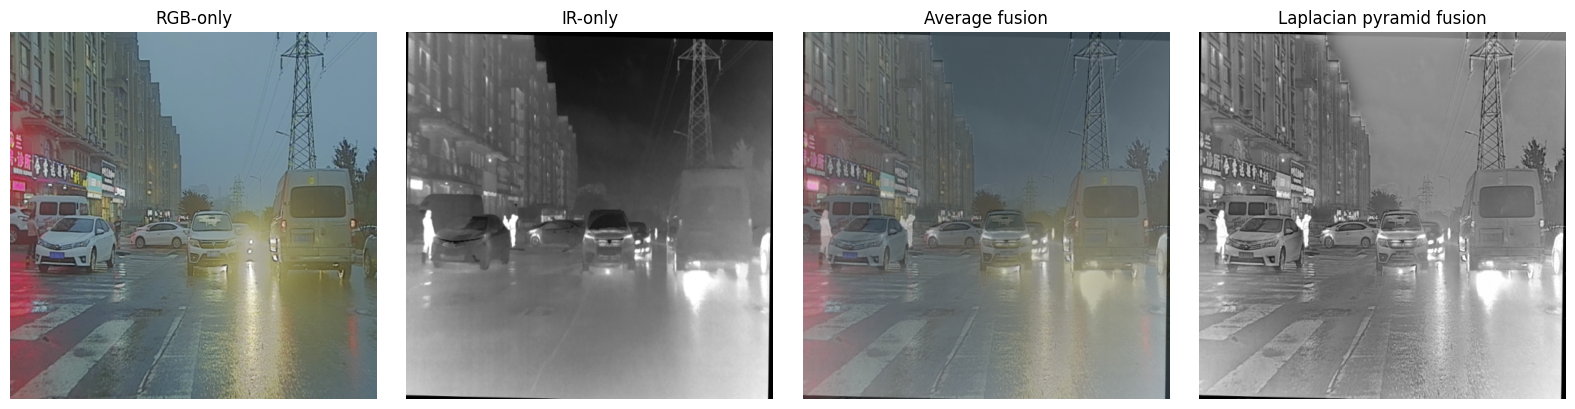
\includegraphics[width=\textwidth]{figures/qualitative_baseline_sample.png}
        \caption{RGB, IR, average, and learned output examples from the notebook.}
    \end{subfigure}\hfill
    \begin{subfigure}[b]{0.48\textwidth}
        \centering
        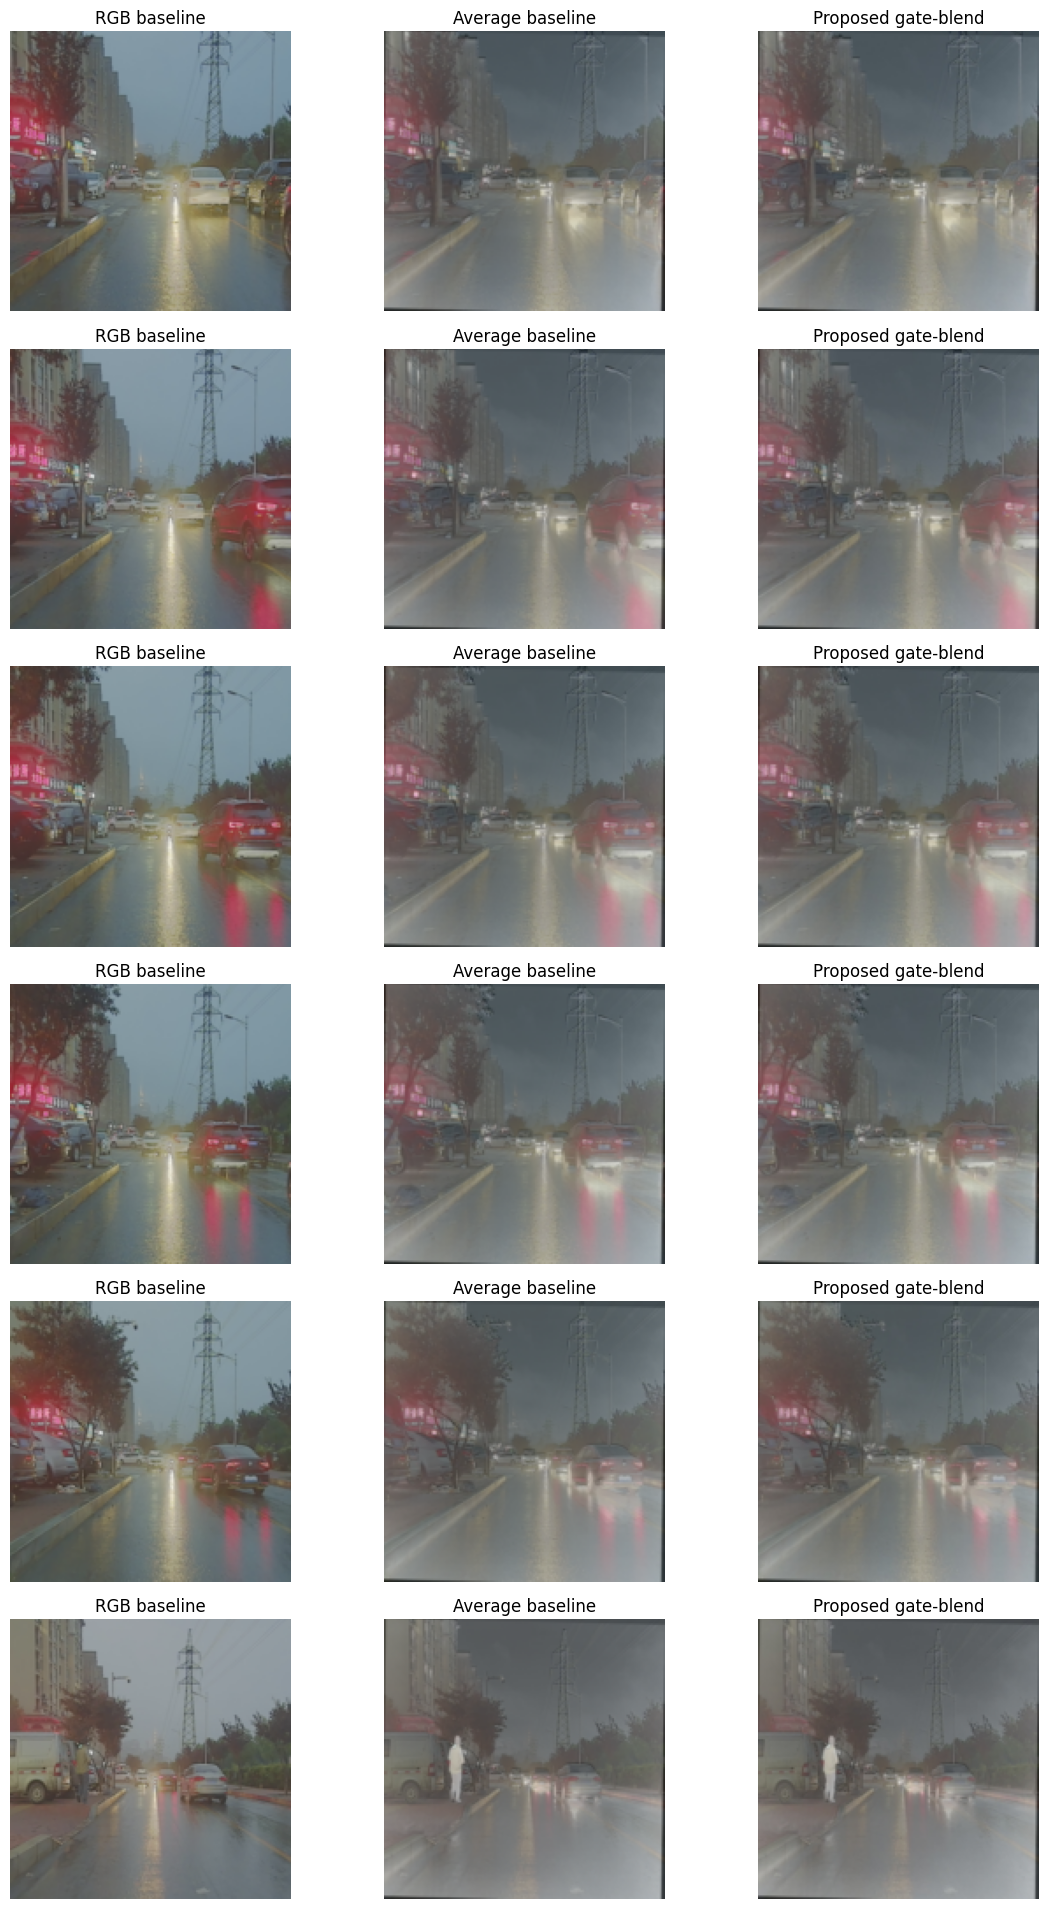
\includegraphics[width=\textwidth]{figures/qualitative_gateblend_sample.png}
        \caption{Corrected gate-blend comparison used for downstream experiments.}
    \end{subfigure}
    \caption{Representative qualitative outputs. The corrected gate-blend output is visually meaningful and avoids the collapsed raw decoder image observed during debugging.}
    \label{fig:qual}
\end{figure*}

\subsection{Object Detection Results}
Table~\ref{tab:downstream} and Fig.~\ref{fig:downstream} summarize the downstream task results. For detection, average fusion achieved the best mAP@0.5 (0.7718) and mAP@0.5:0.95 (0.5115). The proposed CM-JEPA gate-blend method achieved mAP@0.5 = 0.7567 and mAP@0.5:0.95 = 0.5080. It is therefore slightly below average fusion but very close in stricter localization quality. It also improves over IR-only and exceeds RGB-only in mAP@0.5:0.95.

\begin{table}[t]
\centering
\caption{Downstream performance of RGB, IR, average fusion, and the final CM-JEPA gate-blend representation.}
\label{tab:downstream}
\begin{tabular}{lccc}
\toprule
Method & mAP@0.5 & mAP@0.5:0.95 & mIoU \\
\midrule
RGB-only & 0.7616 & 0.4887 & 0.5307 \\
IR-only & 0.7064 & 0.4649 & 0.4976 \\
Average fusion & \textbf{0.7718} & \textbf{0.5115} & \textbf{0.5551} \\
CM-JEPA gate-blend & 0.7567 & 0.5080 & 0.4774 \\
\bottomrule
\end{tabular}
\end{table}

\begin{figure}[t]
    \centering
    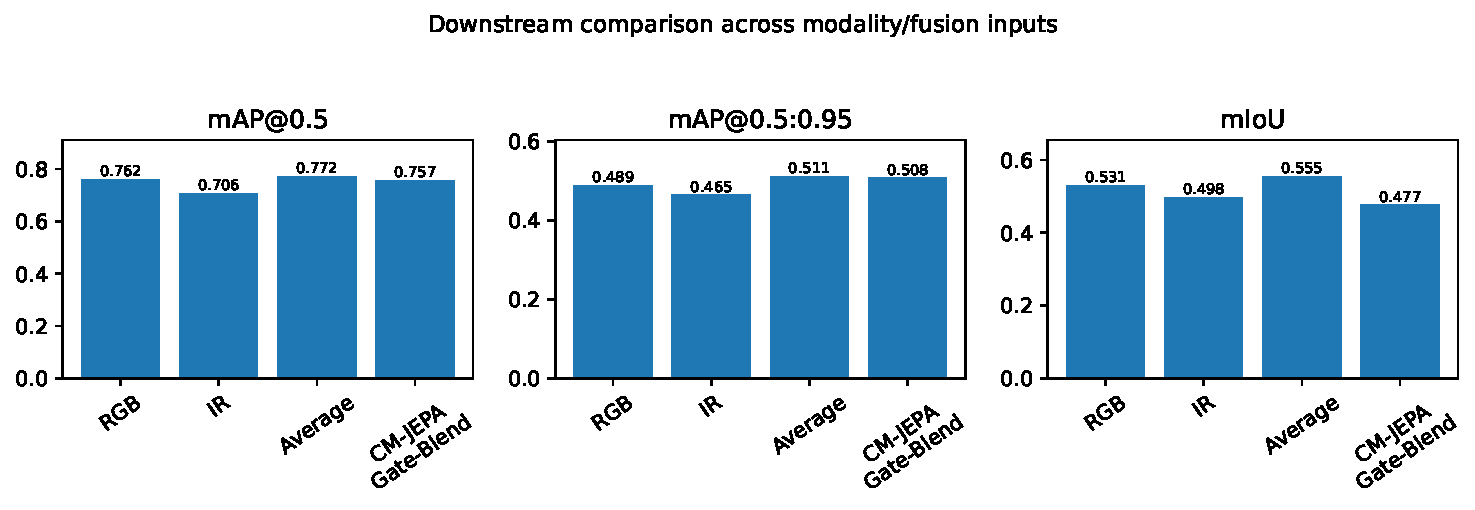
\includegraphics[width=\columnwidth]{figures/figure_downstream_combined.pdf}
    \caption{Downstream results. Average fusion is the best overall method, while CM-JEPA gate-blend is competitive in detection but weak in semantic segmentation.}
    \label{fig:downstream}
\end{figure}

\subsection{Semantic Segmentation Results}
Segmentation reveals a different pattern. Average fusion again achieves the best score with mIoU = 0.5551, followed by RGB-only at 0.5307, IR-only at 0.4976, and CM-JEPA gate-blend at 0.4774. This indicates that the gate-blend representation preserved enough object saliency for detection but did not preserve fine-grained semantic boundaries and textures as effectively as the average baseline. This difference is central to the discussion: detection and segmentation do not require the same kind of visual information.

\subsection{Ablation and Fusion-Quality Metrics}
Table~\ref{tab:ablation} summarizes image-level fusion metrics. The repaired A7 row is particularly important. Before the repair, A7 had zero entropy, spatial frequency, and average gradient because the raw decoder output was being evaluated. After the repair, A7 values became normal and very close to average fusion: EN 6.8898 vs. 6.8732, SF 0.02834 vs. 0.02836, AG 0.01138 vs. 0.01141, and NMI mean 1.1635 vs. 1.1617. This confirms that the final A7 representation behaves similarly to average fusion at the image-statistics level, which is consistent with its near-average detection performance.

\begin{table*}[t]
\centering
\caption{Fusion-quality and ablation metrics. A3-A6 are fusion-only ablation variants; downstream YOLO/U-Net metrics were measured only for A0, A1, A2, and A7.}
\label{tab:ablation}
\begin{tabular}{llcccc}
\toprule
Method & Description & EN & SF & AG & NMI mean \\
\midrule
A0 & RGB-only & 6.2097 & 0.04021 & 0.01517 & 1.5336 \\
A1 & IR-only & \textbf{7.6092} & 0.03879 & 0.01275 & 1.4436 \\
A2 & Average fusion & 6.8732 & 0.02836 & 0.01141 & 1.1617 \\
A3 & Concat, no gate & 7.3225 & 0.01873 & 0.01022 & 1.0744 \\
A4 & No channel attention & 7.3275 & 0.01898 & 0.01038 & 1.0715 \\
A5 & No spatial gate & 7.2397 & 0.01715 & 0.00916 & 1.0805 \\
A6 & Full attention, no JEPA & 7.2156 & 0.01826 & 0.00976 & 1.0754 \\
A7 & Full CM-JEPA gate-blend & 6.8898 & 0.02834 & 0.01138 & 1.1635 \\
\bottomrule
\end{tabular}
\end{table*}

\begin{figure}[t]
    \centering
    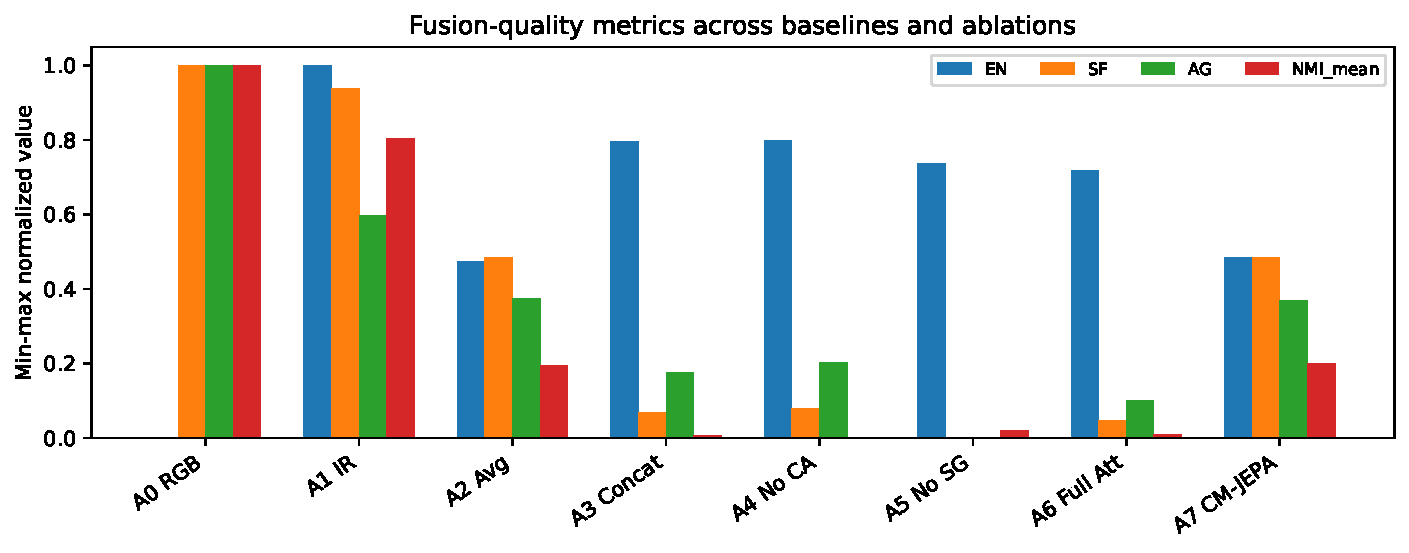
\includegraphics[width=\columnwidth]{figures/figure_fusion_metrics.pdf}
    \caption{Min-max normalized fusion-quality metrics. A7 becomes consistent with average fusion after the gate-blend metric repair.}
    \label{fig:fusionmetrics}
\end{figure}

\subsection{Metric Correlation Analysis}
A correlation analysis was performed between classical fusion metrics and downstream task metrics using the four methods that have both fusion and downstream measurements (A0, A1, A2, A7). Fig.~\ref{fig:corr} shows the updated Pearson correlations after the A7 repair. Because \(n=4\), the p-values are large and the correlations should not be interpreted as statistically conclusive. The qualitative conclusion is still informative: image-level fusion metrics are weak proxies for downstream utility. For example, A7 and average fusion have almost identical EN/SF/AG/NMI values, yet their segmentation mIoU differs substantially. Conversely, IR has high entropy but does not dominate downstream tasks.

\begin{figure}[t]
    \centering
    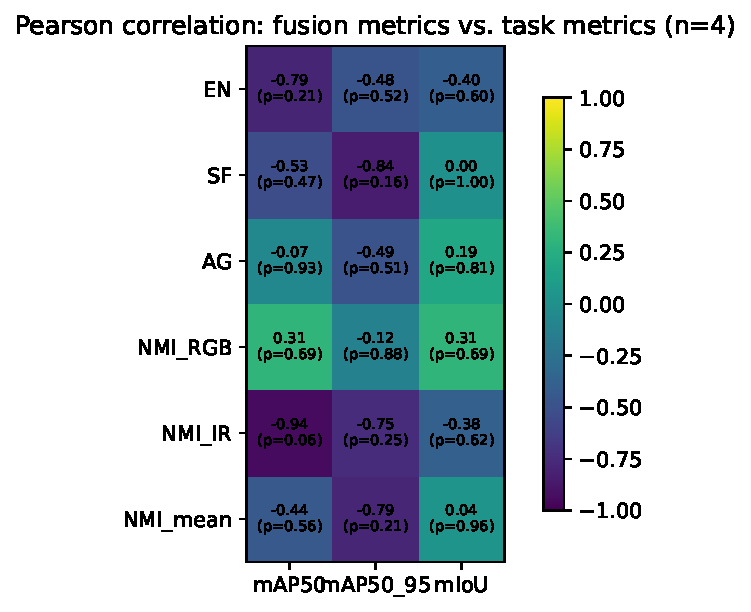
\includegraphics[width=0.95\columnwidth]{figures/figure_correlation_heatmap.pdf}
    \caption{Updated Pearson correlation report after A7 repair. With only four downstream-evaluated methods, the correlations are descriptive rather than statistically conclusive.}
    \label{fig:corr}
\end{figure}

\section{Discussion}
\subsection{What Worked}
The first major finding is that RGB/IR fusion is useful. Average fusion outperformed RGB-only and IR-only in both detection and segmentation. This supports the basic premise of the project: visible and infrared imagery provide complementary information. The improvement is not massive, but it is consistent and meaningful. Detection mAP@0.5 improved from 0.7616 for RGB to 0.7718 for average fusion, and segmentation mIoU improved from 0.5307 to 0.5551.

The second positive result is that the proposed CM-JEPA gate-blend model recovered from the raw-output failure and became detection-competitive. Its mAP@0.5:0.95 score of 0.5080 is nearly equal to average fusion's 0.5115 and higher than RGB-only's 0.4887. This means the learned gate can produce a representation with useful object-level saliency.

\subsection{What Did Not Work as Expected}
The main hypothesis was that a learned attention-based CM-JEPA fusion model would outperform simple fusion. The results do not fully support that claim. Average fusion is the strongest overall method, and CM-JEPA gate-blend fails to improve semantic segmentation. This is a critical result, not an implementation failure. It suggests that adding attention and representation learning does not automatically improve downstream perception. For segmentation, preserving pixel-level semantic boundaries appears more important than generating a visually plausible blend.

The A3-A6 ablation results also show that architectural complexity alone is not enough. These learned variants often have higher entropy than average fusion, but lower spatial frequency and average gradient. They were not downstream-evaluated because doing so would require additional YOLO/U-Net training for every ablation variant. Therefore, they should be interpreted as fusion-quality ablations only. The fair downstream comparison remains A0/A1/A2/A7.

\subsection{Why Detection and Segmentation Behave Differently}
Object detection requires object-level cues: cars, pedestrians, headlights, thermal silhouettes, and bounding-box scale. A fused image can help detection if it makes targets more salient even if some texture is smoothed. Semantic segmentation is stricter. It requires pixel-level class boundaries between road, vegetation, buildings, sky, vehicles, and other classes. A gate-blend image that is adequate for target localization can still damage dense semantic cues. This explains why CM-JEPA gate-blend was competitive for YOLO but weak for U-Net.

\subsection{Why Classical Fusion Metrics Were Insufficient}
Entropy, spatial frequency, average gradient, and mutual information describe image statistics, not task utility. The updated A7 row makes this clear: A7 and average fusion are nearly indistinguishable by EN/SF/AG/NMI, yet average fusion has much higher segmentation mIoU. Thus, fusion-quality metrics should be used as diagnostics, not as substitutes for downstream evaluation. This supports the original proposal's research gap: the relation between pixel-level fusion quality and task performance on lightweight models is weak and must be experimentally tested.

\subsection{Implementation Lessons}
The final code contains two important engineering corrections. First, detection continuation uses saved YOLO exports rather than relying on a fragile global manifest. This prevents MSRS text labels from being mistaken for M3FD detection labels. Second, the proposed representation uses gate-guided blending instead of the raw decoded fused image. The A7 fusion metrics were also repaired to use the same representation as YOLO and U-Net. Without this repair, A7 produced invalid zero-valued fusion metrics. These corrections are documented in the included reproducibility notebook \cite{kulusslu2026notebook}.

\subsection{Limitations}
There are several limitations. First, A3-A6 ablation variants were not propagated through full YOLO and U-Net downstream training due to time and compute cost. Second, the correlation analysis has only four downstream-evaluated methods, so statistical claims are limited. Third, although the dataset is real and multi-source, it still relies on aligned RGB/IR pairs. Misalignment would require additional registration or robustness mechanisms. Fourth, the project uses a 3-channel image adapter so that standard YOLO and U-Net can be reused; a feature-level fusion detector or segmenter could exploit RGB/IR structure more directly.

\section{Conclusion}
This project evaluated cross-modal attention-based RGB/IR fusion with a CM-JEPA component for lightweight detection and segmentation. The final experiments show that RGB/IR fusion is beneficial, but the simplest average fusion is the strongest overall baseline. The proposed CM-JEPA gate-blend representation is detection-competitive and nearly matches average fusion in mAP@0.5:0.95, but it underperforms in semantic segmentation. The repaired A7 fusion metrics show that CM-JEPA gate-blend has image statistics close to average fusion, yet this does not translate into equal segmentation performance. The main conclusion is therefore nuanced: learned RGB/IR gate-blend fusion can be useful for object-level perception, but it does not automatically preserve dense semantic information. Future work should investigate task-aware training with segmentation/detection losses, feature-level downstream fusion, alignment robustness, and a larger downstream ablation set.

\section*{Acknowledgment}
The author used AI tools during the preparation of this study for code debugging assistance, experiment interpretation, writing organization, and LaTeX report drafting. The experimental design decisions, final code execution, result selection, and academic interpretation were reviewed and finalized by the author. Responsibility for the submitted content remains entirely with the author.

\balance
\bibliographystyle{IEEEtran}
\bibliography{references}

\end{document}
